\chapter{Introduction}
\label{C:intro}

Transformer models have been quickly taking over many tasks in the field of deep learning, due to their versatility and proven usefulness. Code completion, image classification, generative art, and many other tasks are being successfully tackled with transformer models.

This thesis provides an introduction to transformer models, presents experiments with new ways of sampling data with them, and then applies them to the domain of hand motion modeling.

\section{Contributions}

Although much of the work done is summarizing others' research and presenting learnings, there are two main novel contributions:
\begin{enumerate}
    \item \Cref{C:a-o-sampling} presents experiments with \textit{dynamically-ordered} auto-regressive sampling, utilising the permutation-invariance property of the attention operation in transformer models. The comparison of different dynamic sampling orders is to my knowledge the first of its kind.
    \item \Cref{C:hand-model} presents proof-of-concept transformer-based generative models for hand motion prediction, which can be used to predict sequences of hand motion conditional on arbitrary target frames. This is a novel application of auto-regressive transformer models, and to my knowledge is the first time that a transformer model has been used on this particular problem of hand joint prediction.
\end{enumerate}
These contributions involved training neural networks (see \Cref{fig:context}), in particular transformers, on two datasets - MNIST, and the ManipNet motion capture dataset \cite{manipnet}. The results of these experiments are presented in \Cref{C:a-o-sampling} and \Cref{C:hand-model} respectively.

\begin{figure}
    \centering
    
\pgfdeclarelayer{bg}
\pgfsetlayers{bg,main}

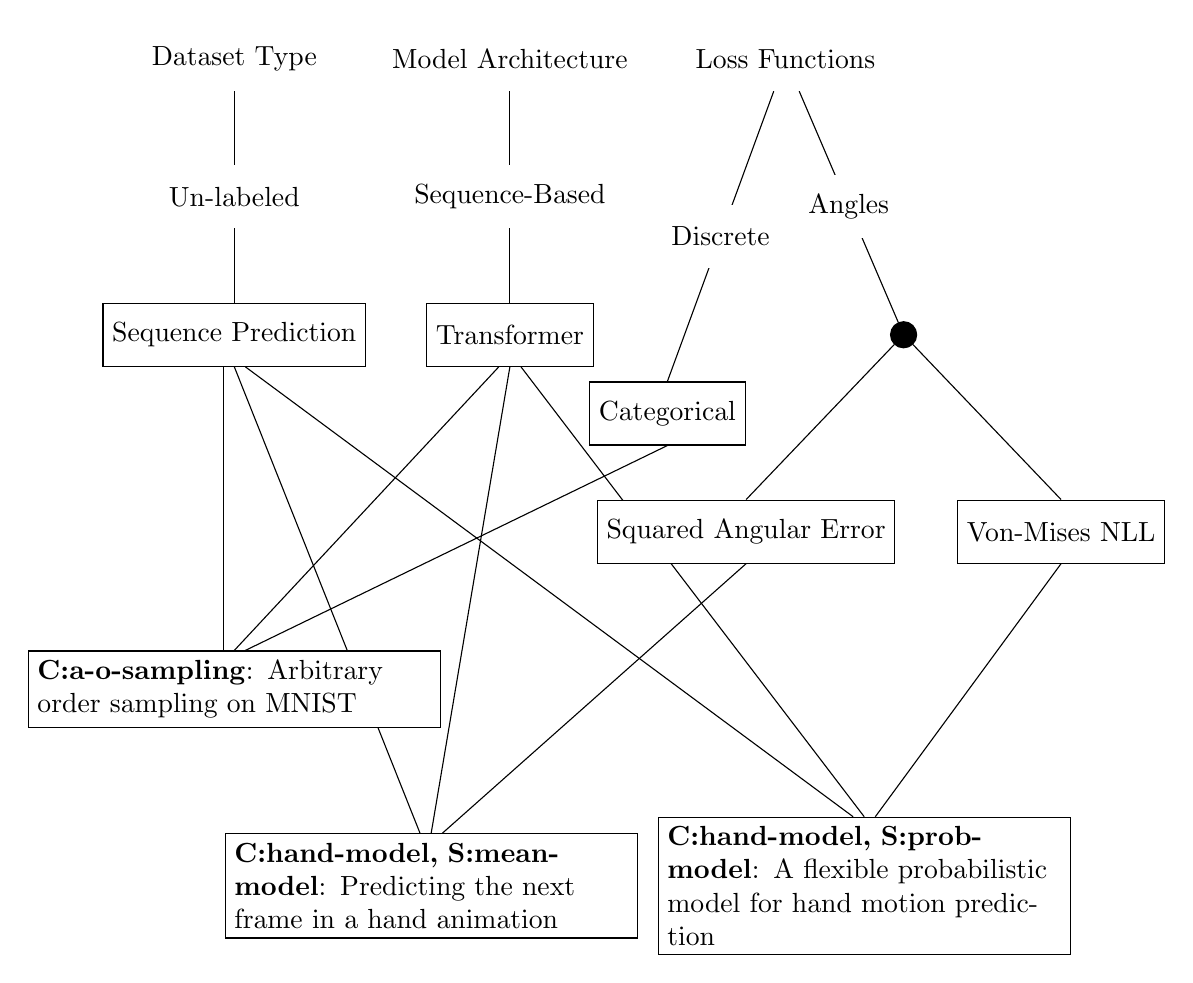
\begin{tikzpicture}
    \tikzstyle{every node}=[node distance=3.5cm,minimum height=0.8cm]

    % dataset type
    \node (datasettype) {Dataset Type};
    \node[draw, below of=datasettype] (seqpred) {Sequence Prediction};
    \draw (datasettype) -- node[fill=white] {Un-labeled} (seqpred);

    % input shape
    \node[right of=datasettype] (seqmodel) {Model Architecture};

    % loss
    \node[right of=seqmodel] (loss) {Loss Functions};

    % angles
    \node[draw,fill=black,minimum height=0.2cm,circle,below of=loss,xshift=1.5cm] (angles) {};
    \draw (loss) -- node[fill=white] {Angles} (angles);

    \node[draw,fill=white,below of=angles,node distance=2.5cm, xshift=-2cm] (amse) {Squared Angular Error};
    \draw (angles) -- (amse.north);

    \node[draw,fill=white,below of=angles,node distance=2.5cm, xshift=2cm] (vonmises) {Von-Mises NLL};
    \draw (angles) -- (vonmises.north);

    \node[draw,fill=white,below of=loss,node distance=4.5cm,xshift=-1.5cm] (cat)  {Categorical};
    \draw (loss) -- node[fill=white] {Discrete} (cat.north);

    % transformer (here because needs to draw above a line)
    \node[draw, below of=seqmodel] (transformer) {Transformer};
    \draw (seqmodel) -- node[fill=white] {Sequence-Based} (transformer);


    % chapter 4: arbitrary order sampling
    \node[draw,fill=white,text width=5cm] (chapter4) at (0,-8cm) {\textbf{\Cref{C:a-o-sampling}}: Arbitrary order sampling on MNIST};

    % chapter 6.2: transformer for hand pose prediction
    \node[draw,fill=white,text width=5cm] (chapter62) at (2.5cm,-10.5cm) {\textbf{\Cref{C:hand-model}, \Cref{S:mean-model}}: Predicting the next frame in a hand animation};

    % chapter 6.3: probabilistic model for hand pose prediction
    \node[draw,fill=white,text width=5cm] (chapter63) at (8cm,-10.5cm) {\textbf{\Cref{C:hand-model}, \Cref{S:prob-model}}: A flexible probabilistic model for hand motion prediction};

    \begin{pgfonlayer}{bg}
        \draw ([xshift=-4pt]seqpred.south) -- ([xshift=-4pt]chapter4.north);
        \draw ([xshift=-4pt]transformer.south) -- (chapter4.north);
        \draw (cat.south) -- ([xshift=4pt]chapter4.north);

        \draw (seqpred.south) -- ([xshift=-4pt]chapter62.north);
        \draw (transformer.south) -- (chapter62.north);
        \draw (amse.south) -- ([xshift=4pt]chapter62.north);

        \draw ([xshift=4pt]seqpred.south) -- ([xshift=-4pt]chapter63.north);
        \draw ([xshift=4pt]transformer.south) -- (chapter63.north);
        \draw (vonmises.south) -- ([xshift=4pt]chapter63.north);
    \end{pgfonlayer}
\end{tikzpicture}

    \vspace{1cm}
    \captionsetup{parskip=7pt}
    \caption[Thesis overview]{How the various concepts in this work are connected to the experiments.

    \Cref{C:a-o-sampling} discusses experiments with different sampling orders for an auto-regressive model trained on the MNIST dataset.

    \Cref{C:hand-model} discusses the development of a model for hand motion modeling using the ManipNet \cite{manipnet} hand motion dataset. \Cref{S:mean-model} focuses on a deterministic model, while \Cref{S:prob-model} focuses on a probabilistic model.}
    \label{fig:context}
\end{figure}

\section{Structure}

The structure of the remainder of the thesis is as follows:

\begin{enumerate}
    \item \Cref{C:background} introduces notation and concepts for neural networks which will be used throughout.

    \item \Cref{C:transformers} provides an introduction and literature review of a class of neural network models called \textit{transformers}, which are a class of models that have become very broadly used in the past few years.

    \item \Cref{C:a-o-sampling} presents a novel method for sampling sequence data in an arbitrary order, including a pre-training task variant, and experiments with this method with transformer models on the MNIST dataset.

    \item \Cref{C:angles-joints-hands} introduces notation and concepts for the problem domain of \textit{hand motion modeling}, including methods for representing and working with joint angles and rotations, and character/hand pose data.

    \item \Cref{C:hand-model} then presents the development of a transformer model for predicting hand pose data and generating animations of hands.

    \item Lastly, \Cref{C:conclusion} summarizes the conclusions of the experiments, and discusses future work and reflections.
\end{enumerate}
